%% ----------------------------------------------------------------
%% main.tex — University of Southampton PhD thesis (phdthesis.cls)
%% ----------------------------------------------------------------
\documentclass[a4paper]{phdthesis}

\usepackage[round]{natbib}
\usepackage{booktabs}

\hypersetup{colorlinks=true}
\graphicspath{{.}}

\renewcommand{\bibname}{References}

% Default fixed font does not support bold face
\DeclareFixedFont{\ttb}{T1}{txtt}{bx}{n}{10} % for bold
\DeclareFixedFont{\ttm}{T1}{txtt}{m}{n}{10}  % for normal

% Custom colors
\usepackage{color}
\definecolor{deepblue}{rgb}{0,0,0.5}
\definecolor{deepred}{rgb}{0.6,0,0}
\definecolor{deepgreen}{rgb}{0,0.5,0}


% Python style for highlighting
\newcommand\pythonstyle{\lstset{
language=Python,
basicstyle=\footnotesize,
otherkeywords={self},             % Add keywords here
keywordstyle=\bfseries\color{black},
emph={MyClass,__init__},          % Custom highlighting
emphstyle=\color{deepred},    % Custom highlighting style
stringstyle=\color{deepgreen},
frame=tb,                         % Any extra options here
showstringspaces=false            % 
}}

% Python environment
\lstnewenvironment{python}[1][]
{
\pythonstyle
\lstset{#1}
}
{}

% Python for external files
\newcommand\pythonexternal[2][]{{
\pythonstyle
\lstinputlisting[#1]{#2}}}

% Python for inline
\newcommand\pythoninline[1]{\text{#1}}


% Algorithm style for highlighting
\newcommand\algstyle{\lstset{
language=Python,
basicstyle=\footnotesize,
otherkeywords={self},             % Add keywords here
keywordstyle=\bfseries\color{black},
emph={MyClass,__init__},          % Custom highlighting
emphstyle=\color{black},    % Custom highlighting style
stringstyle=\color{black},
frame=tb,                         % Any extra options here
showstringspaces=false,            % 
captionpos=t
}}


% Algorithm environment
\lstnewenvironment{algorithm}[1][]
{
\algstyle
\lstset{#1}
}
{}


%% ----------------------------------------------------------------
\begin{document}
\frontmatter
\title      {Reduced-Order Models for Real-Time Cardiovascular Flow Simulation}
\date       {June 2026}
\author     {Sarah J. Whitfield}
\supervisor {Prof. Nigel Bressloff}
\university {University of Southampton}
\department {Computational Engineering and Design}
\group      {Computational Engineering and Design Group}
\faculty    {Faculty of Engineering and Physical Sciences}

\maketitle

\begin{abstract}
Full three-dimensional computational fluid dynamics simulations of blood
flow are too slow to use in a clinical setting, where results are often
needed within minutes. This thesis develops a reduced-order one-dimensional
blood flow model that captures pulse wave propagation through the major
arteries at a fraction of the computational cost of a full 3D simulation.
We validate the model against 3D simulations and in vivo measurements
across a range of vessel geometries, and show that it reproduces pressure
and flow waveforms with clinically acceptable accuracy while running
several orders of magnitude faster, making real-time patient-specific
simulation feasible.
\end{abstract}

\tableofcontents
\listoffigures
\listoftables
\lstlistoflistings
\listofsymbols{llc}{
$p$ & pressure & Pa\\
$q$ & volumetric flow rate & m$^3$/s\\
$A$ & cross-sectional area & m$^2$\\
$c$ & pulse wave velocity & m/s}
\listofacronyms{ll}{
CFD & Computational Fluid Dynamics\\
1D & One-Dimensional\\
ROM & Reduced-Order Model}
\declaration{Whitfield, S.J. (2026). Parts of Chapter 2 have been presented at the International Conference on Computational Biomechanics.}
\acknowledgements{I thank my supervisor for his guidance throughout this project, and the Computational Engineering and Design Group for many helpful discussions. This work was supported by an EPSRC studentship.}
\mainmatter
%% ----------------------------------------------------------------
\chapter{Introduction}

Computational fluid dynamics (CFD) simulations of blood flow through the
arterial network can take hours to run even on modern hardware, which
makes them impractical for use during a clinical consultation, where a
decision may need to be made within minutes \citep{Diem2017a}.

\section{Motivation}
Reduced-order one-dimensional (1D) blood flow models approximate the full
3D Navier-Stokes equations by averaging over the vessel cross-section,
trading some spatial detail for a very large reduction in computational
cost \citep{Diem2017b}. Prior 1D models have been validated primarily
against idealised geometries rather than patient-specific vessel networks.

\section{Contributions}
This thesis makes the following contributions:
\begin{itemize}
  \item A reduced-order 1D blood flow model validated against full 3D CFD
    simulations across a range of patient-specific vessel geometries.
  \item A comparison against in vivo pressure and flow measurements from
    an existing clinical dataset.
  \item An analysis of the run-time and accuracy trade-off relative to
    full 3D simulation, showing the model is fast enough for real-time
    use at a clinically acceptable accuracy.
\end{itemize}

\begin{figure}
  \center
  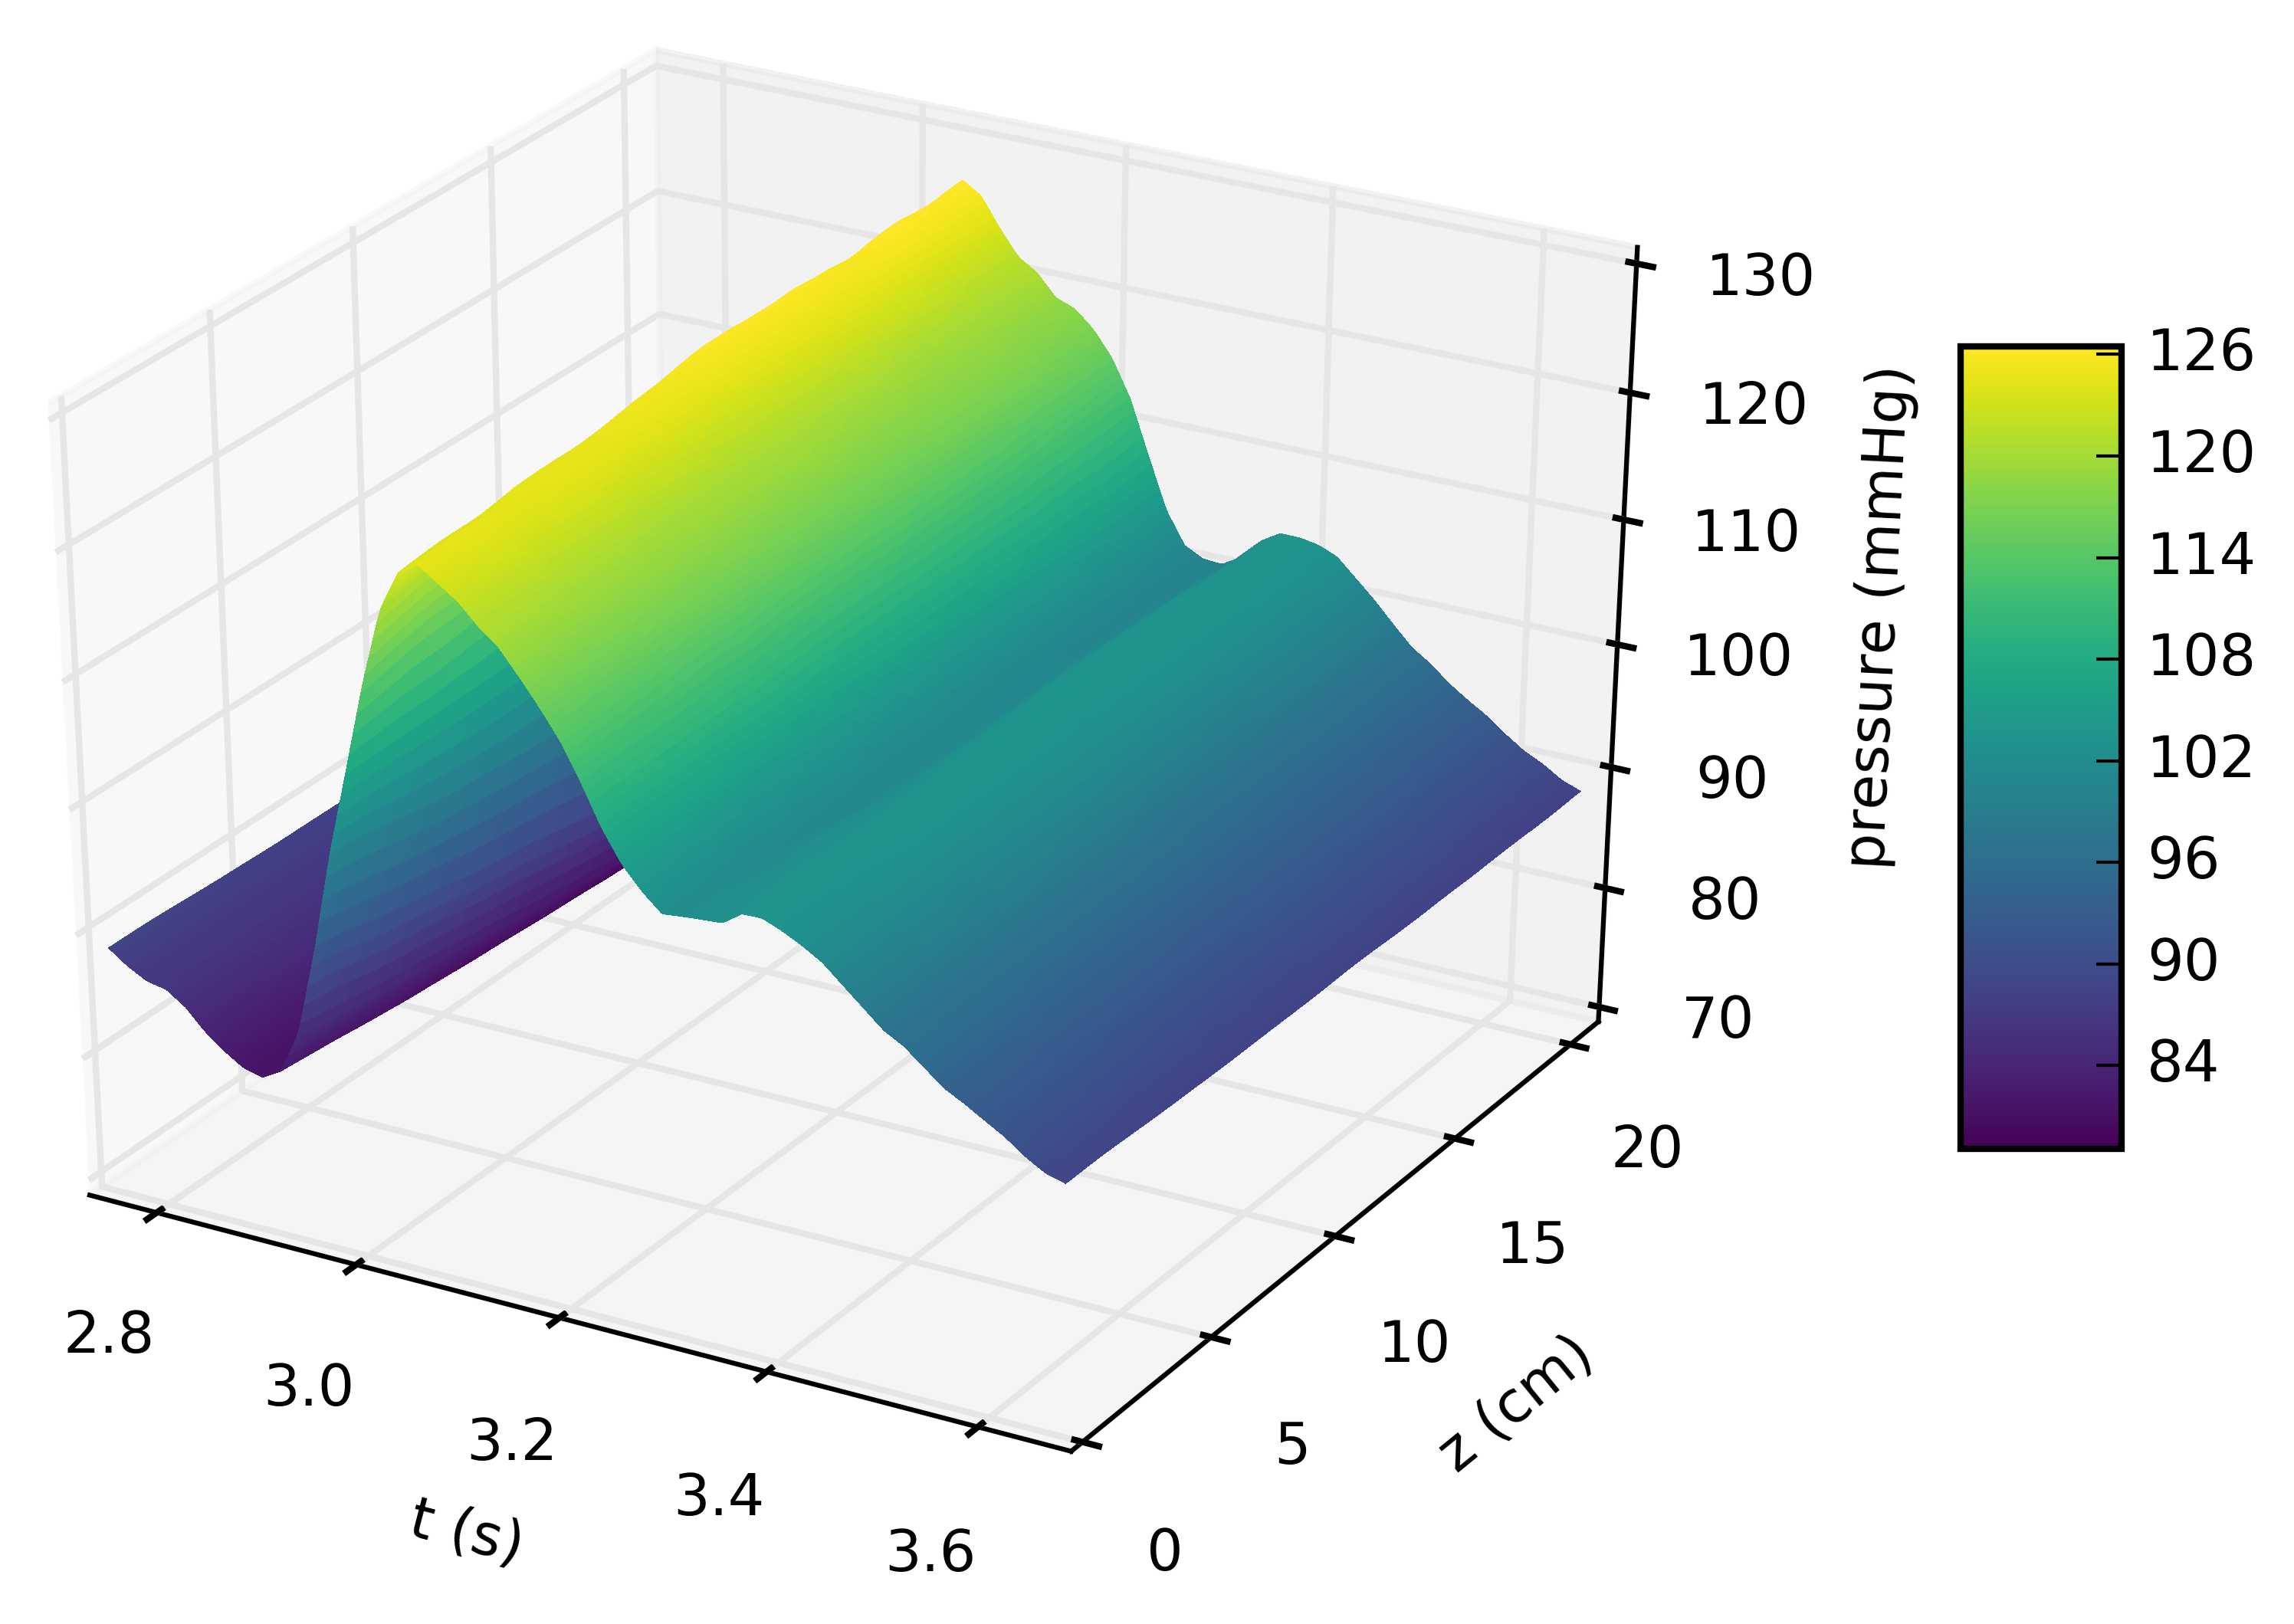
\includegraphics[width=0.6\linewidth]{figure.png}
  \caption{Illustrative one-dimensional discretisation of an arterial segment.\label{fig:1}}
\end{figure}

It references \fref{fig:1}.

\begin{table}
  \center
  \caption{Vessel segments included in the validation dataset.\label{tab:1}}
  \begin{tabular}{cc}
    \toprule
    Segment & Number of Cases\\
    \midrule
    Aorta & 12\\
    Carotid & 9\\
    Femoral & 7\\
    \bottomrule
  \end{tabular}
\end{table}

It also references \tref{tab:1}.

\chapter{Method}

This chapter describes the one-dimensional model formulation and the
numerical scheme used to solve it.

\begin{figure}
  \begin{algorithm}[caption={One time step of the explicit finite-volume update.}, label=alg:1]
    for segment in vessel_network:
        flux_left = compute_flux(segment.left_state)
        flux_right = compute_flux(segment.right_state)
        segment.state -= dt / segment.dx * (flux_right - flux_left)
  \end{algorithm}
\end{figure}

It references \aref{alg:1}.

The core update step can also be prototyped directly in Python:

\begin{python}
def update_segment(state, flux_left, flux_right, dt, dx):
    return state - dt / dx * (flux_right - flux_left)
\end{python}

We validate the numerical scheme against an analytical solution for
pulse wave propagation in a single straight vessel before applying it to
the full patient-specific network \citep{Diem2017a,Diem2017b}.


\appendix
\chapter{Model Parameters}

This appendix would list the vessel wall stiffness and reference radius
parameters used for each vessel segment in the validation dataset,
omitted from this starter document.


%% ----------------------------------------------------------------
\backmatter
\bibliographystyle{plainnat}
\bibliography{references}
\end{document}
%% ----------------------------------------------------------------
